\section{Introduction}
Typically, segregation is measured using groups of individuals assigned to organizational units. A segregation index is a mathematical function that maps the joint distribution of groups and organizational units into $\mathbb{R}^+$. Traditional measures, such as the dissimilarity \citep{duncan_duncan_1955} or the Gini \citep{fluckiger_silber_1999} indices, are appropriate for computing segregation when (i) there are two groups and (ii) the organizational units lack a hierarchical or multilevel structure.

One classic example from the segregation literature addresses measuring segregation among Black and White students in schools. However, even in this simple scenario, there may be information in the data that calls for a less restrictive use of the indices.
First, there are often multiple sources of identity and affiliation that may result in nondichotomous groups \citep{akerlof_kranton_2010}. For example, ethnic classification may include more than two categories. Additionally, the definition of groups can be extended by operating a Cartesian product among multiple sources of segregation: ethnicity, gender, religion, income, and language are consequential factors defining group membership in many societies. In this case, we would need to use a multigroup segregation index \citep{reardon2002measures}.

Second, we may hypothesize that multigroup ethnic segregation in schools is produced via two channels. One is the segregation between the ethnic majority and the remainder. The second channel is the segregation among minorities. In this scenario, we should be interested in decomposing the overall value of a segregation index into (i) a ``between'' term (gauging segregation in schools between the majority and the minorities) and (ii) a ``within'' term (computing segregation among the minorities). An index that satisfies the so-called \textit{strong group decomposability} (\textit{SGD}) property achieves this goal in the best possible way \citep{frankel_volij_2011}.

We are also interested in another multilevel structure of the situation. For example, in many countries, schools belong to districts, and district authorities may have powers over the assignment of students to schools. We should examine: (i) how much ethnic segregation is in districts and (ii) how much is in schools. For this, we'll break down the total segregation into that of larger areas (districts) and specific units (schools). Complying with the so-called \textit{strong unit decomposability} (\textit{SUD}) property addresses this goal \citep{frankel_volij_2011}.

As far as we know, the mutual information or $M$ index---originally proposed to study race segregation in Chicago's public schools \citep{theil_finizza_1971}---is the only multigroup segregation index that simultaneously satisfies the two abovementioned properties.

There are two packages in R to compute $M$ and its decompositions. First, the \code{mutual\_total} function of the \CRANpkg{segregation} package \citep{segregation-package} computes the index itself and the ``within'' term of the decomposition. By calling \code{mutual\_total} twice, we obtain a simple ``between''-``within''  decomposition.\footnote{This package has additional features not directly related to the decompositions discussed in this paper. It (i) computes local segregation scores; (ii) uses bootstrap procedures to conduct inferential analyses; (iii) decomposes pairwise comparisons of indices to solve the problem of marginal dependence; and (iv) computes the $H$ index, which is a normalization of the $M$ index.} Second, in this article, we present the \CRANpkg{mutualinf} package \citep{mutualinf-package} for computing complex ``between''-``within'' decompositions, i.e., decompositions with multiple ``within'' terms.

In the next section, we introduce the $M$ index and its decomposability properties. Next, we illustrate its usage with an application to a Chilean school enrollment dataset. We then explain the package structure. The last section summarizes the main contributions of the \CRANpkg{mutualinf} package.

\section{Statistical model}
Consider two discrete random variables, $unit$ and $group$. Let $p_{ng}$ represent the joint proportion of individuals for whom $unit=n$ and $group=g$. Then, 
\begin{equation}
P_{unit, group} = \{p_{ng}| \forall n \in 1,\ldots,N, \forall g \in 1,\ldots,G\} \label{eq: joint}
\end{equation}
denotes the joint distribution of the discrete random variables $unit$ and $group$, and $\sum_{n=1}^{N} \sum_{g=1}^{G} p_{ng} = 1$. 

In addition, let $p_{n \bullet} = \sum_{g=1}^{G}p_{ng}$ such that
\begin{equation}
P_{unit} = \{p_{n\bullet}| \forall n \in 1,\ldots,N\} \label{eq: marg_unit}
\end{equation}
denotes the marginal distribution of individuals across units. Similarly, let $p_{\bullet g} = \sum_{n=1}^{N} p_{ng}$, and
\begin{equation}
P_{group} = \{p_{\bullet g}| \forall g \in 1,\ldots,G\} \label{eq: marg_group}
\end{equation}
be the marginal distribution across groups. Finally, let
\begin{equation}
P_{unit|g} = \left\{\frac{p_{ng}}{ p_{\bullet g}}| \forall g \text{ and } n\right\} \label{cond_g}
\end{equation}
and
\begin{equation}
P_{group|n} = \left\{\frac{p_{ng}}{ p_{n\bullet}}| \forall g \text{ and } n\right\} \label{cond_n}
\end{equation}
be the conditional distributions across units and groups. 

The $M$ index is the weighted average of the natural logarithm of the ratio between (i) the actual joint distribution of units and groups and (ii) the joint distribution under the hypothesis of independence or no association.

\begin{equation}
    M = \sum_{g=1}^{G} \sum_{n=1}^{N} p_{ng} \log{ \left( \frac{p_{ng}}{p_{n \bullet} p_{\bullet g}} \right),}
    \label{eq: M-definition}
\end{equation}
where we set $0 \times \log_{b} \left( \frac{1}{0} \right) = 0$. For simplicity, the $M$ index uses the natural logarithm, although any base will work:

\begin{equation}
    M_b = \frac{M}{\log_e{\left(b\right)}}.
    \label{eq: M-base-change}
\end{equation}

As a measure of association, the index captures the excess uncertainty that exists when we learn about someone's unit and group separately rather than jointly. When groups and units are independent, the joint proportions $p_{ng}$ equal the proportions under independent assignment: $p_{ng} = p_{n \bullet} p_{\bullet g}$.\footnote{It can be shown that the $M$ index is a monotonic transformation of the likelihood ratio test of random assignment across units and groups \citep{zoloth_1974}.} Then, naturally, $M=0$. Note that this is the minimum of the index. In effect, the $M$ index is nonnegative and less than or equal to the logarithm of $\min \{G,N\}$. Often, $G < N$; and so the index reaches its maximum value, $\log(G)$, whenever equal-sized groups are isolated in separate units.

The $M$ index builds on the concept of entropy from information theory \citep{kullback_1959}: the average information attained when we learn the value of a discrete variable.
\citet{frankel_volij_2011} characterize $M$ with six ordinal axioms.
Interestingly, and rather conveniently, the $M$ index can be expressed in two different but equivalent ways that represent two notions of segregation that \citet{massey_denton_1988} propose: segregation as the average departure of (i) $P_{group | n}$ from $P_{group}$ and (ii) of $P_{unit | g}$ from $P_{unit}$.

\subsection{Decomposability properties}
Social scientists who study sources of segregation should use an index that satisfies either \textit{SUD} or \textit{SGD} or both depending on whether the interest lies in sources stemming from units, groups, or both \citep{mora_ruiz-castillo_2003, frankel_volij_2011, mora2011entropy}.

Let $S$ be an \textit{SUD} index of segregation defined over variables $group$ and $unit$. Consider a partition of all the units, $n=1,\ldots,N,$ into $K$ major units, $k=1,\ldots,K$. Let $S_{K}$ be the index of segregation that we obtain after taking the $K$ major units as organizational units. $S_K$ is usually referred to as the ``between'' term. Following \citet{frankel_volij_2011}, we decompose an \textit{SUD} index as:
\begin{equation}
    S = S_{K} + \sum_{k=1}^{K} p_{k \bullet} S(k),
    \label{eq: SUD-property}
\end{equation}
\noindent where $p_{k \bullet}$ is the demographic share of major unit $k$, and $S(k)$ is the segregation index of major unit $k$. With an \textit{SUD} index, the following scenario holds: if the differences in group proportions across the units of each major unit $k$ vanished but the differences in group proportions across major units remained, segregation would decrease by the amount in $\sum_{k=1}^{K} p_{k \bullet} S(k)$. (The latter expression is commonly referred to as the ``within'' term.)
In other words, $\sum_{k=1}^{K} p_{k \bullet} S(k)$ represents the exclusive contribution of $unit$ segregation that arises within major units (e.g., school segregation within districts); therefore, it is unrelated to segregation that arises in major units \citep{mora2011entropy}. Conversely, for a partition of $group$, we can decompose an \textit{SGD} index into a ``between'' and a ``within'' term following a similar procedure.

As mentioned above, we can study sources of segregation \texttt{only} with indices that satisfy the \textit{SUD} and/or \textit{SGD} properties. Consider, for example, the situation in which the Cartesian product of several discrete variables define $group$. Let $A$ be the subset of all the variables defining $group$. If index $S$ satisfies the \textit{SGD} property, we can decompose it $\text{card}(A)$ times. Each decomposition would take the categories resulting from excluding one variable at a time as the major groups. Denote $S(A\backslash j),\forall j\in A$ as the ``within'' term in the decomposition that takes the Cartesian product of all the variables in $A{\backslash j}$ as supergroups. This term, $S(A{\backslash j})$, identifies the exclusive contribution of the variable $j$ to the overall group segregation in variable $unit$. For notational simplicity, let us express this as follows:

\begin{equation}
    S^j:=S\left(A{\backslash j}\right).
    \label{eq:contribution_j}
\end{equation}
In general, $S\neq\sum_{j=1}^{J}S^j$. We can always define:
\begin{equation}
    I = S - \sum_{j=1}^{J}S^j.
    \label{eq: interaction-term-definition}
\end{equation}
Therefore, $I\in \mathbb{R}$ can be interpreted as the ``interaction'' among all the variables in $A$, i.e., the slack or surplus in $S$ that cannot exclusively be attributed to any variable in $A$. Hence:
\begin{equation}
    S =  \sum_{j=1}^{J}S^j + I.
    \label{eq: SGD-property}
\end{equation}

Conversely, with index $S$ satisfying \textit{SUD}, we can study the segregation stemming from variable $unit$. If $S$ satisfies both \textit{SGD} and \textit{SUD}, we can identify the exclusive contributions to overall segregation that come from all variables defining $group$ \textit{and} $unit$.
The contributions of the $group$ variables are computed on the segregation defined along all $unit$ variables. Conversely, the contributions of the $unit$ variables are computed on the segregation defined using all the $group$ variables. Correspondingly, the resulting conceptual framework does not allow for simultaneously measuring the contributions of the $group$ and $unit$ variables. Nonetheless, it is possible to compute the segregation that stems from a subset of the $unit$ and $group$ variables.

The $M$ index is the only multigroup segregation index that is known to satisfy the $SUD$ and $SGD$ properties simultaneously and that can, therefore, implement decompositions \ref{eq: SUD-property} and \ref{eq: SGD-property}.

%This section may contain a figure such as Figure~\ref{figure:rlogo}.

%\begin{figure}[htbp]
  %\centering
  %
\includegraphics{Rlogo}
  %\caption{The logo of R.}
  %\label{figure:rlogo}
%\end{figure}

\section{Illustration of \CRANpkg{mutualinf} with school data}
We illustrate the use of \CRANpkg{mutualinf} with Chilean school enrollment data from the 2016-2018 period. The data include all students ($n =$ 287,546) in the schools of the regions of Biobío, La Araucanía, and Los Ríos. These are the three administrative regions with the largest proportion of Mapuche people, the main ethnic minority in Chile.

We merged three datasets using unique student identifiers and enrollment years. \textit{Datos Abiertos}, ``Open Data'' in Spanish, (Ministry of Education, \url{https://datosabiertos.mineduc.cl/}) is the main dataset. It includes individual-level information about all the students enrolled in grades/years 4 and 8 (\code{grade}). This includes their school (\code{school}), enrollment/academic year (\code{year}), gender (\code{gender}), and whether they receive (partially or fully) the government means-tested allowance for students (\code{csep}, the acronym of ``preferential student allowance'' in Spanish \textit{subvención escolar preferencial}).\footnote{The criteria for receiving a full or partial subsidy during the period 2016-2018 are closely related to the socioeconomic level of the student's family. Hence, the type of student subsidy received by each student is a proxy for his or her socioeconomic status, SES. In particular, students who receive no allowance are high SES students; students who receive partial allowance are middle SES students; and students with full allowance are low SES students.} A total of 168,684 (58.7\%) students received either the partial or full allowance.
Moreover, the data include school-level information: the school ID (there are 2,454 schools), the school's ownership status (public, private, or charter;  \code{sch\_type}), rural or urban location (\code{rural}), administrative district (there are 98 administrative districts; \code{district}), and region (the three regions abovementioned; \code{region}).

The two other datasets are the \textit{Cuestionario de Calidad y Contexto de la Educación para Padres y Apoderados} (``Quality and Education Survey for Parents and Guardians'') and the \textit{Cuestionario de Estudiantes} (``Student Survey'', Education Quality Agency, \url{https://www.agenciaeducacion.cl/}).
With them, we construct a proxy for belonging to the Mapuche ethnic minority (\code{ethnicity}): we classify a student as Mapuche if he or she, or at least one parent, self-identifies as such. With this, the broadest possible definition of the Mapuche group with these data, there are 41,884 (14.6\%) Mapuche students in the sample\footnote{According to the Chilean Statistical Office, in the 2017 Census 12.8 percent of the population consider themselves to belong to one of the native peoples of the country. The ``Quality and Education Survey for Parents and Guardians'' and the ``Student Survey'' record only whether a student self-identifies as a member of a native group. Still, the Mapuches account for over 99 percent of the native population in the three regions that we study \citep{instituto2018radiografia}.}



\begin{table}
\begin{tabular}{@{}
p{0.15\textwidth} p{0.81\textwidth}
@{}}
\toprule
Variable & Description \\
\\
\multicolumn{2}{l}{\emph{Individual Characteristics}}\\
\code{year} & Student enrollment/academic year.\\
\code{gender} & Student gender code.\\
\code{csep} & Preferential student allowance category. \\
\code{grade} & Student grade/year.  \\
\code{ethnicity} & Self-reported Native ethnicity. \\
\\
\multicolumn{2}{l}{\emph{School Characteristics}}\\
\code{school} & School ID. \\
\code{district} & Administrative district where the school is located. \\
\code{region} & Administrative region where the school is located. \\
\code{rural} & School with multiage classrooms. \\% Rafa, esto es 1 para rural?
\code{sch\_type} & Whether the school is public, charter, or private. \\

\bottomrule
\end{tabular}
\caption{Variable definitions. Individual-level enrollment data, 2016--2018, Biobío, La Araucanía, and Los Ríos regions (Chile).}
\label{tbl: variables-description}
\end{table}

\begin{comment}
\begin{table}
\centering
\begin{tabular}{@{}
p{0.1\textwidth} p{0.1\textwidth}  p{0.1\textwidth}
p{0.17\textwidth} p{0.12\textwidth} p{0.1\textwidth}@{}}
\toprule
    &      & \multicolumn{3}{c}{Region}  &  \\ \cmidrule{3-5}
    &       & Biobio & La Araucania & Los Rios & Total \\
    \midrule
            & 2016 & 56860  & 28057        & 10733  &   95650   \\
    year    & 2017 & 56445  & 28111        & 10712  &   95268 \\
            & 2018 & 57081  & 28665        & 10882  &   96628  \\
            \cmidrule{2-6}
            & Total & 170386    & 84833 & 32327 &   287546 \\
\bottomrule
\end{tabular}
\caption{Students by Region and Year}
\label{tbl: students-by-year-and-region}
\end{table}

\begin{table}[!ht]
\centering
\begin{tabular}{@{}
p{0.17\textwidth} p{0.1\textwidth}  p{0.1\textwidth}
p{0.17\textwidth} p{0.12\textwidth}  p{0.1\textwidth}@{}}
\toprule
    &      & \multicolumn{3}{c}{Region}     \\ \cmidrule{3-5}
    &       & Biobio & La Araucania & Los Rios  & Total \\
    \midrule
                & public    & 81014     & 33452     & 16116 & 130582 \\
    sch\_type   & charter   & 82181     & 48850     & 14961 & 145992 \\
                & private   & 7191      & 2531      & 1250  & 10972 \\
                \midrule
    rural   & urban     & 149004    & 67263 & 24541 & 240808 \\
            & rural     & 21382     & 17570 & 7786  & 46738 \\
\bottomrule
\end{tabular}
\caption{Students by Region, School Type, and Rural/Urban Status}
\label{tbl: school-classification}
\end{table}


\begin{table}[!ht]
\centering
\begin{tabular}{@{}
p{0.12\textwidth} p{0.18\textwidth}  p{0.1\textwidth}
p{0.17\textwidth} p{0.12\textwidth} p{0.1\textwidth}@{}}
\toprule
    &      & \multicolumn{3}{c}{Region}     \\ \cmidrule{3-5}
    &       & Biobio & La Araucania & Los Rios  & Total \\
    \midrule
            & subsidized         & 48151 & 20232 & 8351  & 76734 \\
    CSEP    & partially subsidized       & 94794 & 54210 & 19680 & 168684 \\
            & unsubsidized    & 27441 & 10391 & 4296  & 42128 \\
            \midrule
    ethnicity   & non-Mapuche    & 157467    & 62583 & 25612    & 245662 \\
                & Mapuche       & 12919     & 22250 & 6715      & 41884 \\
                \midrule
    gender  & female    & 86947 & 43262 & 16517 & 146726 \\
            & male      & 83439 & 41571 & 15810 & 140820 \\
            \midrule
    grade   & 4    & 85179 & 42475 & 16295  & 143949 \\
            & 8   & 85207 & 42358 & 16032   & 143597 \\
\bottomrule
\end{tabular}
\caption{Students by Allowance Status, Ethnicity, Gender, and Grade [aka `year']}
\label{tbl: students-classification}
\end{table}
\end{comment}

\subsection{School segregation}

In this section, we work with the aggregated school enrollment data described in Table \ref{tbl: variables-description}. First, we load the package \CRANpkg{mutualinf}. The \code{data.table} function of this package automatically allows us to use our examples (\code{DT\_Seg\_Chile}):\footnote{The  categories for the variable \code{csep} in \code{DT\_Seg\_Chile} have been modified so that the table fits the margins: \code{s} for \code{subsidized}, \code{ps} for \code{partially-subsidized}, and \code{ns} for \code{non-subsidized}.}

\begin{example}
> library(mutualinf)
\end{example}
\vfill
\begin{example}
> DT_Seg_Chile
       year school district csep   ethnicity rural   region sch_type gender grade fw

    1: 2016   4531     8101   ps non-Mapuche urban   Biobio   public female     4 22
    2: 2016   4531     8101    s non-Mapuche urban   Biobio   public female     4 19
    3: 2016   4531     8101    s     Mapuche urban   Biobio   public female     4  2
    4: 2016   4531     8101   ns non-Mapuche urban   Biobio   public female     4  5
    5: 2016   4531     8101   ps     Mapuche urban   Biobio   public female     4  2
   ---                                                                                              
55956: 2018  22495    14204   ps non-Mapuche urban Los Rios  charter   male     8  1
55957: 2018  22495    14204   ps     Mapuche urban Los Rios  charter   male     8  2
55958: 2018  22495    14204    s     Mapuche urban Los Rios  charter   male     8  5
55959: 2018  22495    14204   ns non-Mapuche urban Los Rios  charter   male     8  1
55960: 2018  22495    14204   ns     Mapuche urban Los Rios  charter   male     8  1
\end{example}

Each row in the database is a unique combination of the values that the variables in Table \ref{tbl: variables-description} take, representing a subset of the students.
The last column, \code{fw}, contains the number of students enrolled in each unique subset. The remaining columns correspond to the variables in Table \ref{tbl: variables-description}.

The \code{mutual} function can calculate the $M$ index at its simplest level, i.e., as a measure of group segregation in a set of units.  For example, suppose that the objective is to compute the $M$ index of socioeconomic school segregation. In that case, schools define the units, and the preferential student allowance categories (proxies of socioeconomic status) define the three socioeconomic groups. The following code computes socioeconomic segregation in schools:
\begin{example}
> mutual(data = DT_Seg_Chile,
         group = "csep",
         unit = "school")
           M
1: 0.1995499
\end{example}

As previously stated, $\log(\min(G,N))$ is the upper bound of
the $M$ index. Hence, a given index value represents different segregation
levels depending on $G$ and $N$. Normalization can help in this
situation. Given that there are only three socioeconomic groups but
many more schools, the upper bound in this case is $\log(3)\approx1.0986$.
We can use this value to normalize $M$, i.e., to rescale its value
as a proportion of maximum segregation: $0.1995/1.0986=0.1816$ or,
in other words, in our data, socioeconomic groups generate only $0.1816\times100=18.16\%$ of the maximum segregation that there could be. The cardinality of \emph{any} normalized index, i.e., the index value we calculate with it, only warrants this limited interpretation. However, it comes at a high price for the normalized $M$ index because it no longer satisfies the $SGD$ property. Conversely, if the upper bound were defined by $N$, the resulting normalized index would no longer satisfy the $SUD$ property \citep{mora2021computing}.

To return to our example, we can also compute ethnic segregation in schools:

\begin{example}
> mutual(data = DT_Seg_Chile,
         group = "ethnicity",
         unit = "school")
            M
1: 0.06213906
\end{example}

The \code{mutual} function can also take on board multiple group dimensions. For example, we can measure socioeconomic \textit{and} ethnic segregation in schools:
\begin{example}
> mutual(data = DT_Seg_Chile,
         group = c("csep", "ethnicity"),
         unit = "school")
           M
1: 0.2610338
\end{example}
In the above example, the \code{mutual} function defines groups as combinations of socioeconomic and ethnic categories.
By design, the value of the overall segregation thus obtained (\code{0.2610338}) must be greater than or equal to the value for the segregation measured for socioeconomic or ethnic groups separately: \code{0.1995499} and \code{0.06213906}, respectively.
Note that \code{0.1995499} (\code{0.06213906}) is the value of the ``between'' term in the decomposition of the total segregation in schools (\code{0.2610338}) that there is within socioeconomic (ethnic) categories. Given that the ``within'' term must be nonnegative, it follows that the ``between'' term cannot be greater than total segregation.

More generally, segregation analyses can be computed using a variety of unit- and/or group-defining variables. For example,
\begin{example}
> mutual(data = DT_Seg_Chile,
         group = c("csep", "ethnicity"),
         unit = c("school", "district"))
           M
1: 0.2610338
\end{example}
computes the socioeconomic and ethnic segregation in combinations of schools and districts. Note that the result, \code{0.2610338}, is identical to that obtained in the previous case. The reason is that each school belongs to only one district; hence, the combinations of schools and districts coincide with the set of schools. This occurs because the two variables are hierarchically related and districts partition schools. In other words, districts do not add information about segregation beyond what is obtained from schools.

However, the variables that define the units may not lie in a hierarchy. For example, defining the units with the school identification code (\code{school}) and ownership type (\code{sch\_type}), we obtain a different value for the overall socioeconomic and ethnic segregation:
\begin{example}
> mutual(data = DT_Seg_Chile,
         group = c("csep", "ethnicity"),
         unit = c("school", "sch_type"))
           M
1: 0.2610865
\end{example}
Why is this so? It turns out that a few schools changed ownership during the sample period, making for a nonhierarchical relationship between \code{school} and \code{sch\_type}, the two unit-defining variables. The consequence is a slight increase in the overall measure of socioeconomic and ethnic segregation from 0.261033 to 0.2610865 that is entirely due to the enlargement of the set of units from schools to the combination of schools and ownership type.

Setting the option \code{by} allows us to compute the index for subsets of \code{data} separately. In our database, the variable \code{region} partitions \code{data} into three regions:
\begin{example}
> mutual(data = DT_Seg_Chile,
        group = c("csep", "ethnicity"),
        unit = c("school", "sch_type"),
        by = "region")
         region         M
1:       Biobio 0.2312423
2: La Araucania 0.2367493
3:     Los Rios 0.2125013
\end{example}
The segregation in La Araucania is greater than that in either Biobio or Los Rios. By including more than one variable in option \code{by}, the subsets are defined by the Cartesian product of the categories of these variables. To illustrate it, we include the variables \code{region} and \code{year} to option \code{by}:
\begin{example}
> mutual(data = DT_Seg_Chile,
           group = c("csep", "ethnicity"),
           unit = c("school", "sch_type"),
           by = c("region", "year"))
         region year         M
1:       Biobio 2016 0.2423257
2:       Biobio 2017 0.2599383
3:       Biobio 2018 0.2696983
4: La Araucania 2016 0.2818232
5: La Araucania 2017 0.2749189
6: La Araucania 2018 0.2873032
7:     Los Rios 2016 0.2489342
8:     Los Rios 2017 0.2540016
9:     Los Rios 2018 0.2664027
\end{example}
In the above example, we obtain a segregation index for each combination of region and year: the socioeconomic segregation and ethnic segregation in Biobio and Los Rios increase during the sample period (2016-2018); however, the segregation in La Araucania falls in 2017 and grows in 2018.

The \code{within} option additively decomposes the total segregation index into a ``between'' and a ``within'' term. We return to the \code{by="region"} example:
\begin{example}
> mutual(data = DT_Seg_Chile,
         group = c("csep", "ethnicity"),
         unit = c("school", "sch_type"),
         by = "region",
         within = "ethnicity")
         region         M M_B_ethnicity M_W_ethnicity
1:       Biobio 0.2312423    0.02582674     0.2054156
2: La Araucania 0.2367493    0.04840892     0.1883404
3:     Los Rios 0.2125013    0.03324738     0.1792539
\end{example}
We obtain three terms for each region. The first, \code{M}, contains total segregation and matches the values without the \code{within} option. The second, \code{M\_B\_ethnicity}, contains values for the ``between'' term that measures ethnic segregation in the combinations of schools and types of schools. The third, \code{M\_W\_ethnicity}, contains values for the ``within'' term. These values are the weighted averages of the socioeconomic segregation (in the combinations of schools and types of schools) computed for each ethnic group (with weights equal to the demographic importance of each ethnicity). This ``within'' term is the part of the total segregation, \code{M}, that stems exclusively from socioeconomic differences. Hereafter, we will refer to these ``within'' terms, which isolate sources of segregation,  as ``contributions''. In this case, \code{M\_W\_ethnicity} is the socioeconomic contribution to total segregation \code{M}.

It is also possible to decompose the \code{M} index into a ``between'' and a ``within'' socioeconomic term:
\begin{example}
> mutual(data = DT_Seg_Chile,
         group = c("csep", "ethnicity"),
         unit = c("school", "sch_type"),
         by = "region",
         within = "csep")
         region         M  M_B_csep   M_W_csep
1:       Biobio 0.2312423 0.2030819 0.02816039
2: La Araucania 0.2367493 0.1906641 0.04608521
3:     Los Rios 0.2125013 0.1774420 0.03505928
\end{example}
Now, we obtain, again, three terms for each region. The first, \code{M}, captures total segregation as before. The second, \code{M\_B\_csep}, is the socioeconomic segregation in the combinations of schools and types of schools. The third, \code{M\_W\_csep}, is the ethnic contribution.

The \code{within} option also allows us to sequentially conduct more than one decomposition, using either major units and/or supergroups. Consider parsing the combinations of \code{csep}, \code{ethnicity}, and \code{gender} as supergroups:
\begin{example}
> mutual(data = DT_Seg_Chile,
         group = c("csep", "ethnicity", "gender"),
         unit = c("school", "grade"),
         by = "region",
         within = c("csep", "ethnicity"))
         region         M  M_B_csep      M_W_csep M_W_csep_ethnicity
1:       Biobio 0.3026811 0.2086340    0.04019188         0.05385515
2: La Araucania 0.3261384 0.1970565    0.07945498         0.04962692
3:     Los Rios 0.3328145 0.1833409    0.06585940         0.08361417
\end{example}
In the above output, we obtain four terms for each region. The first, \code{M}, is the socioeconomic, ethnic, and gender segregation in the combinations of schools and grades, i.e., in the organizational units. The second, \code{M\_B\_csep}, is the socioeconomic segregation in the combinations of schools and grades. The third, \code{M\_W\_csep}, presents the weighted average across all socioeconomic levels of ethnic segregation in schools and grades. (This term is not the contribution of ethnicity because it also includes the interaction between ethnicity and gender.) The fourth, \code{M\_W\_csep\_ethnicity}, is the contribution of gender to total segregation. Note that labels \code{M\_W\_csep} and \code{M\_W\_csep\_ethnicity} are shortcuts for \code{M\_W\_csep\_B\_ethnicity} and \code{M\_W\_csep\_W\_ethnicity\_B\_gender}, respectively.

Returning to the example without gender, we can directly obtain contributions using the \linebreak \code{contribution.from} option. Take the following example:
\begin{example}
> mutual(data = DT_Seg_Chile,
         group = c("csep", "ethnicity"),
         unit = c("school", "sch_type"),
         by = "region",
         contribution.from = "group_vars")
         region         M    C_csep C_ethnicity  interaction
1:       Biobio 0.2312423 0.2054156  0.02816039 -0.002333648
2: La Araucania 0.2367493 0.1883404  0.04608521  0.002323710
3:     Los Rios 0.2125013 0.1792539  0.03505928 -0.001811897
\end{example}
Following Equations~\eqref{eq:contribution_j} and \eqref{eq: interaction-term-definition}, we obtain four terms for each region: \code{M}, \code{C\_csep}, \code{C\_ethnicity}, and \code{interaction}. \code{M} is total segregation, as already presented. \code{C\_csep} is the socioeconomic contribution. It matches the ``within'' ethnicity term (\code{M\_W\_ethnicity}) in the first \code{within} example above. \code{C\_ethnicity} is the ethnic contribution. It matches the ``within'' socioeconomic term (\code{M\_W\_csep}) in the second \code{within} example above. Finally, \code{interaction} is equal to \code{M} minus the sum of \code{C\_csep} and \code{C\_ethnicity}, as defined in Equation~\eqref{eq: interaction-term-definition}. In other words, the interaction is the part of the total socioeconomic and ethnic segregation that exists in the combinations of schools and school types that cannot exclusively be attributed to either socioeconomic status or ethnicity. The socioeconomic contribution is largest in Biobio (\code{0.2054156}), and the ethnicity contribution is largest in La Araucania (\code{0.04608521}).

A positive interaction term, such as the one in La Araucania, signals that socioeconomic status and ethnicity are sources pushing segregation together in the same direction. Many authors employ the term \textit{intersectionality} to refer to this sort of ``double disadvantage'' scenario, where people from a poor minority are more segregated from the rest than they would be if they were only poor or from an ethnic minority (\citealp{crenshaw1990mapping}).

By contrast, a negative interaction term, as that for Biobio and Los Rios, reflects that socioeconomic status and ethnicity pull in opposite directions: their effects cancel each other out to a certain extent. This situation has been reported empirically previously \citep{guinea2015joint}. However, it remains undertheorized in the literature on the multidimensional nature of social inequality and segregation. 

We can perform the same analysis conditional on group variables using the option \code{within}:

\begin{example}
> mutual(data = DT_Seg_Chile,
         group = c("csep", "ethnicity"),
         unit = c("school", "sch_type"),
         by = "region",
         within = "ethnicity",
         contribution.from = "unit_vars")
         region         M M_B_ethnicity  C_school   C_sch_type interaction
1:       Biobio 0.2312423    0.02582674 0.1053177 3.885868e-05  0.10005903
2: La Araucania 0.2367493    0.04840892 0.1276039 7.777505e-06  0.06072869
3:     Los Rios 0.2125013    0.03324738 0.1065172 7.811955e-05  0.07265861
\end{example}

In the above output, there are five terms for each region. The first term, \code{M}, matches the first term in the previous example. The second term, \code{M\_B\_ethnicity}, contains measures of ethnic segregation in schools and school types. The following two columns, (\code{C\_school} and \code{C\_sch\_type}), are the contributions of schools and school types, respectively, to socioeconomic segregation after controlling for ethnic segregation. The last term, \code{interaction}, is the part of segregation that cannot exclusively be attributed to either schools or their ownership types.

The \code{contribution.from} option can also be used to display the contributions of a subset of variables. For example,
\begin{example}
> mutual(data = DT_Seg_Chile,
         group = c("csep", "ethnicity"),
         unit = c("school", "sch_type"),
         by = "region",
         contribution.from = "csep")
         region         M    C_csep 
1:       Biobio 0.2312423 0.2054156 
2: La Araucania 0.2367493 0.1883404 
3:     Los Rios 0.2125013 0.1792539 
\end{example}
returns \code{M} and \code{C\_csep}.

The contributions can also be displayed for organizational units. Take the following example:
\begin{example}
> mutual(data = DT_Seg_Chile,
         group = c("csep", "ethnicity"),
         unit = c("school", "sch_type"),
         by = "region",
         contribution.from = "unit_vars")
         region         M  C_school   C_sch_type interaction
1:       Biobio 0.2312423 0.1293566 4.860549e-05  0.10183706
2: La Araucania 0.2367493 0.1709480 8.563946e-06  0.06579272
3:     Los Rios 0.2125013 0.1351602 1.903942e-04  0.07715072
\end{example}
The first column in the above output holds measures of total segregation, \code{M}, as before. The second column, \code{C\_school}, contains the contributions of schools. The third column, \code{C\_sch\_type}, contains the contribution of ownership type. The fourth column, \code{interaction}, is the part of socioeconomic and ethnic segregation that cannot exclusively be attributed to segregation in either schools or by ownership type. As previously stated, most schools in the sample period retain their ownership type, so each school can almost uniquely be classified by its \code{sch\_type}. Hence, ownership is a negligible source of information.

The display of the contributions is simpler when variables are hierarchically related:
\begin{example}
> mutual(data = DT_Seg_Chile,
         group = c("csep", "ethnicity"),
         unit = c("school", "district"),
         by = "region",
         contribution.from = "unit_vars")
         region         M  C_school C_district interaction
1:       Biobio 0.2311937 0.1558457          0  0.07534802
2: La Araucania 0.2367407 0.1635589          0  0.07318187
3:     Los Rios 0.2123109 0.1605696          0  0.05174127
\end{example}
The contribution of districts, \code{C\_district}, is zero because each school is in only one district; consequently, there is no segregation by district within schools.

The analysis of contributions using option \code{contributions.from} can be generalized to situations with more than two sources of segregation on either the group or the unit dimension but not both (see the Statistical Model section). For example, in the following code, we consider three sources of group segregation as given by the variables \code{csep}, \code{ethnicity}, and \code{gender}:
\begin{example}
> mutual(data = DT_Seg_Chile,
         group = c("csep", "ethnicity", "gender"),
         unit = c("school", "sch_type"),
         by = "region",
         contribution.from = "group_vars")
         region         M    C_csep C_ethnicity   C_gender interaction
1:       Biobio 0.2732082 0.2143819  0.03442763 0.04196586 -0.01756726
2: La Araucania 0.2718253 0.2017662  0.05742349 0.03507595 -0.02244036
3:     Los Rios 0.2838373 0.1942702  0.04659460 0.07133600 -0.02836349
\end{example}
In the output, there are columns for total segregation (\code{M}), the contributions of each of the three sources of group segregation (\code{C\_csep}, \code{C\_ethnicity}, and \code{gender}), and the interaction term. Total segregation increases when the students' gender is considered. It is the highest in Los Rios (\code{0.2838373}).

In the index decompositions, the ``within'' terms are weighted averages of local indices with demographic weights. To assess the relative importance of demographic weights versus local indices, we set the option \code{components=TRUE}.
\begin{example}
> mutual(data = DT_Seg_Chile,
         group = c("csep", "ethnicity"),
         unit = c("school", "sch_type"),
         within = "csep",
         components = TRUE)
$Total
           M  M_B_csep   M_W_csep
1: 0.2610865 0.1995741 0.06151239

$W_Decomposition
                   csep         p     within
1: partially-subsidized 0.2668582 0.04907351
2:           subsidized 0.5866331 0.07331278
3:       non-subsidized 0.1465087 0.03691946
\end{example}

In the element labeled \code{W\_Decomposition}, we obtain all the components of the linear combination that constitutes the ``within'' term. In particular, we obtain (i) the demographic weights (\code{p}) and (ii) the indexes of ethnic segregation in schools and ownership type (\code{within}) for each of the three socioeconomic groups (\code{csep}) in the data. The average of \code{within}, weighted by \code{p}, is the value of the ``within'' term displayed in the output labeled \code{\$Total}, i.e., \code{M\_W\_csep}: 0.06151239. By inspecting the components of the within term, we conclude that students who obtain the full allowance drive the ``within'' term: they are both (i) the largest demographic group and (ii) the group where ethnic segregation in schools and ownership type is the highest.

\section{Package structure}
The \CRANpkg {mutualinf} package requires \CRANpkg {data.table} \citep{data.table} to speed up data processing. The package provides two functions. The first, \code{prepare\_data}, allows the user to convert a microdata file to a multidimensional frequency table of the \code{data.table} and \code{mutual.data} classes. The \code{mutual} function calculates and decomposes the $M$ index. Figure \ref{figure:diagram-1} represents the package graphically, showing the relationships between the objects and functions of the package.

\begin{figure}[H]
  \centering
  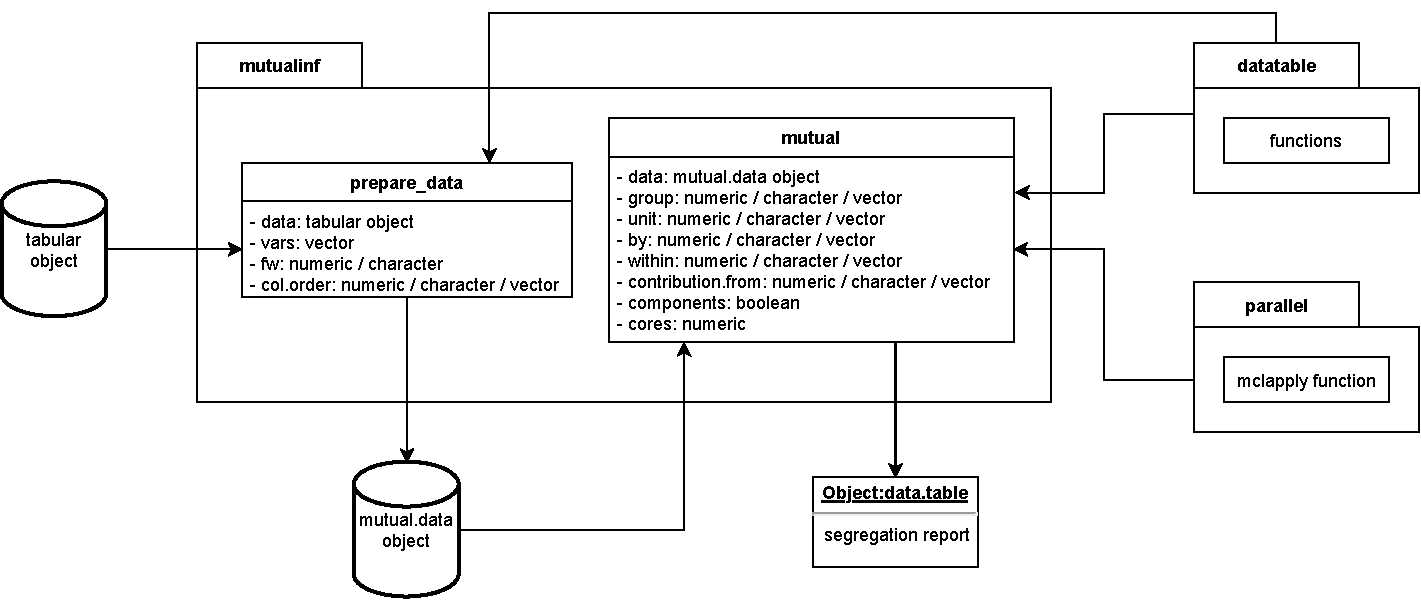
\includegraphics[width=\textwidth]{diagram_v3.pdf}
  \caption{Package structure}
  \label{figure:diagram-1}
\end{figure}

\begin{algorithm}[H]
\caption{\small \code{mutual\_within}}\label{alg:mutual_within}
\small
\begin{algorithmic}
\Require \code{data},\code{group},\code{unit},\code{within},\code{by},$i$,$p_{k \bullet}$,$result$
\If{$i==1$}
    \State $result \gets \emptyset$
    \State Compute $M$ for the first variable of \code{within} (the $between$ term)
    \State Compute $p_{k \bullet}$
    \State Remove the first variable from \code{within} and append it to \code{by}
    \State $i \gets i+1$
    \State Append to $result$ the $between$ term
    \State Append to $result$ mutual\_within(\code{data},\code{group},\code{unit},\code{within},\code{by},$i$,$p_{k \bullet}$,$result$)
    \Return $result$
\ElsIf{\code{within}$\,==\emptyset$}     
    \State $M_k \gets \emptyset$
    \For{$k \in$ the Cartesian product of the variables in \code{by}}
        \State Append to $M_k$ the $M$ for $k$
    \EndFor
    \If{i>2}
        \State Subtract the dot product between $p_{k \bullet}$ and $M_k$ from the last element in $result$
    \EndIf
    \State Append to result the dot product between $p_{k \bullet}$ and $M_k$
    \Return $result$
    \Else
        \State $M_k \gets \emptyset$
        \For{$k \in$ the Cartesian product of the variables in \code{by}}
              \State Append to $M_k$ the $M$ for $k$
        \EndFor
        \If{i>2}
            \State Subtract the dot product between $p_{k \bullet}$ and $M_k$ from the last element in $result$
        \EndIf
        \State $i \gets i+1$
        \State Append to $result$ the dot product between $p_{k \bullet}$ and $M_k$ 
        \State Remove the first variable from \code{within} and append it to \code{by}
        \State Compute $p_{k \bullet}$
        \State Append to $result$ mutual\_within(\code{data},\code{group},\code{unit},\code{within},\code{by},$i$,$p_{k \bullet}$,$result$)
        \Return $result$
\EndIf
\end{algorithmic}
\end{algorithm}

Depending on its parameters, the \code{mutual} function carries out three different levels of analysis---basic, intermediate, and advanced---and outputs either indices alone or indices and their components. 

At its most basic level, the algorithm computes the $M$ index. In its first level of analysis, the \code{mutual} function computes the index using the variables that define groups and units established by the parameters \code{group} and \code{unit}, respectively. In its second level, \code{mutual} generates subsets (identified by the \code{by} parameter) on which it computes the index.

At the intermediate degree of complexity, \code{mutual} performs ``between'' and ``within'' decompositions of the index. In its first level, %\code{mutual} calls Algorithm \ref{alg:mutual_within} to
computes the decomposition %by setting a 
with a single variable in the \code{within} parameter. If this variable belongs to the \code{unit} parameter, the function computes the decomposition that is shown in Equation~\eqref{eq: SUD-property} by applying the \textit{SUD} property. Conversely, if this variable belongs to the \code{group} parameter, the function computes the decomposition that relies on the \textit{SGD} property. 
In its second level, \code{mutual} generates subsets over the vector of variables defined in the \code{by} parameter. It then computes the index and its decompositions for each subset. 

At its highest complexity, \code{mutual} allows for multiple decompositions. In its first level of analysis, it computes the index and decompositions for each element in the \code{within} parameter.%, again, calling Algorithm \ref{alg:mutual_within}. 
In its second level, the function generates subsets using the \code{by} parameter and computes the index and its multiple decompositions for each subset.

In Algorithm \ref{alg:mutual_within}, we illustrate the recursive calculation of all the terms in a decomposition by groups or units. This algorithm receives as inputs \code{data}, the dataset or  multidimensional frequency table processed with \code{prepare\_data}; \code{group}, the set of variables that identify the groups; \code{unit}, the set of variables that identify the units; \code{within}, the set of variables in which the index is decomposed; \code{by}, the set of variables that identify the subsets of the dataset; $i$, a control variable to identify if the decomposition is the first one performed; $p_{k \bullet}$, the demographic weights of the subsets obtained with \code{by}; and $result$, the variable that contains the output of the algorithm. See that $result$ is both an input and an output variable due to the recursive implementation of the algorithm. 

\section{Conclusions}
In this paper, we introduce the \CRANpkg{mutualinf} package that implements a general approach for using the strong decomposability properties of the mutual information index in R. \CRANpkg{mutualinf} exploits both recursion and parallelization techniques to facilitate the chained computation of ``within'' terms in complex decompositions of the index. We use Chilean primary school enrollment data to illustrate the usefulness and flexibility of the package. Of all the sources of segregation in schools considered, socioeconomic differences among students constitute the main source. The contributions to the overall segregation of ethnicity and gender are substantially lower.

\section{Availability}
The package is available in CRAN \url{https://cran.r-project.org/web/packages/mutualinf/}. The development version is available in GitHub \url{https://github.com/RafaelFuentealbaC/mutualinf}.

\section{Acknowledgement}
Rafael Fuentealba-Chaura and Julio Rojas-Mora acknowledge the financial support by the FONDECYT/ANID Project 11170583. Ricardo Mora and Daniel Guinea-Martin acknowledge the financial support of MCIN/AEI/10.13039/501100011033 (Project no. PID2019-108576RB-I00). Cluster time was provided by the UCT VIP Project FEQUIP2019-INRN-03.
